\documentclass[preprint, 3p,
authoryear]{elsarticle} %review=doublespace preprint=single 5p=2 column
%%% Begin My package additions %%%%%%%%%%%%%%%%%%%

\usepackage[hyphens]{url}

  \journal{A Journal} % Sets Journal name

\usepackage{lineno} % add

\usepackage{graphicx}
%%%%%%%%%%%%%%%% end my additions to header

\usepackage[T1]{fontenc}
\usepackage{lmodern}
\usepackage{amssymb,amsmath}
\usepackage{ifxetex,ifluatex}
\usepackage{fixltx2e} % provides \textsubscript
% use upquote if available, for straight quotes in verbatim environments
\IfFileExists{upquote.sty}{\usepackage{upquote}}{}
\ifnum 0\ifxetex 1\fi\ifluatex 1\fi=0 % if pdftex
  \usepackage[utf8]{inputenc}
\else % if luatex or xelatex
  \usepackage{fontspec}
  \ifxetex
    \usepackage{xltxtra,xunicode}
  \fi
  \defaultfontfeatures{Mapping=tex-text,Scale=MatchLowercase}
  \newcommand{\euro}{€}
\fi
% use microtype if available
\IfFileExists{microtype.sty}{\usepackage{microtype}}{}

\ifxetex
  \usepackage[setpagesize=false, % page size defined by xetex
              unicode=false, % unicode breaks when used with xetex
              xetex]{hyperref}
\else
  \usepackage[unicode=true]{hyperref}
\fi
\hypersetup{breaklinks=true,
            bookmarks=true,
            pdfauthor={},
            pdftitle={Catch Composition by Position of Hook in Water Column},
            colorlinks=false,
            urlcolor=blue,
            linkcolor=magenta,
            pdfborder={0 0 0}}

\setcounter{secnumdepth}{5}
% Pandoc toggle for numbering sections (defaults to be off)

% Pandoc syntax highlighting
\usepackage{color}
\usepackage{fancyvrb}
\newcommand{\VerbBar}{|}
\newcommand{\VERB}{\Verb[commandchars=\\\{\}]}
\DefineVerbatimEnvironment{Highlighting}{Verbatim}{commandchars=\\\{\}}
% Add ',fontsize=\small' for more characters per line
\usepackage{framed}
\definecolor{shadecolor}{RGB}{248,248,248}
\newenvironment{Shaded}{\begin{snugshade}}{\end{snugshade}}
\newcommand{\AlertTok}[1]{\textcolor[rgb]{0.94,0.16,0.16}{#1}}
\newcommand{\AnnotationTok}[1]{\textcolor[rgb]{0.56,0.35,0.01}{\textbf{\textit{#1}}}}
\newcommand{\AttributeTok}[1]{\textcolor[rgb]{0.77,0.63,0.00}{#1}}
\newcommand{\BaseNTok}[1]{\textcolor[rgb]{0.00,0.00,0.81}{#1}}
\newcommand{\BuiltInTok}[1]{#1}
\newcommand{\CharTok}[1]{\textcolor[rgb]{0.31,0.60,0.02}{#1}}
\newcommand{\CommentTok}[1]{\textcolor[rgb]{0.56,0.35,0.01}{\textit{#1}}}
\newcommand{\CommentVarTok}[1]{\textcolor[rgb]{0.56,0.35,0.01}{\textbf{\textit{#1}}}}
\newcommand{\ConstantTok}[1]{\textcolor[rgb]{0.00,0.00,0.00}{#1}}
\newcommand{\ControlFlowTok}[1]{\textcolor[rgb]{0.13,0.29,0.53}{\textbf{#1}}}
\newcommand{\DataTypeTok}[1]{\textcolor[rgb]{0.13,0.29,0.53}{#1}}
\newcommand{\DecValTok}[1]{\textcolor[rgb]{0.00,0.00,0.81}{#1}}
\newcommand{\DocumentationTok}[1]{\textcolor[rgb]{0.56,0.35,0.01}{\textbf{\textit{#1}}}}
\newcommand{\ErrorTok}[1]{\textcolor[rgb]{0.64,0.00,0.00}{\textbf{#1}}}
\newcommand{\ExtensionTok}[1]{#1}
\newcommand{\FloatTok}[1]{\textcolor[rgb]{0.00,0.00,0.81}{#1}}
\newcommand{\FunctionTok}[1]{\textcolor[rgb]{0.00,0.00,0.00}{#1}}
\newcommand{\ImportTok}[1]{#1}
\newcommand{\InformationTok}[1]{\textcolor[rgb]{0.56,0.35,0.01}{\textbf{\textit{#1}}}}
\newcommand{\KeywordTok}[1]{\textcolor[rgb]{0.13,0.29,0.53}{\textbf{#1}}}
\newcommand{\NormalTok}[1]{#1}
\newcommand{\OperatorTok}[1]{\textcolor[rgb]{0.81,0.36,0.00}{\textbf{#1}}}
\newcommand{\OtherTok}[1]{\textcolor[rgb]{0.56,0.35,0.01}{#1}}
\newcommand{\PreprocessorTok}[1]{\textcolor[rgb]{0.56,0.35,0.01}{\textit{#1}}}
\newcommand{\RegionMarkerTok}[1]{#1}
\newcommand{\SpecialCharTok}[1]{\textcolor[rgb]{0.00,0.00,0.00}{#1}}
\newcommand{\SpecialStringTok}[1]{\textcolor[rgb]{0.31,0.60,0.02}{#1}}
\newcommand{\StringTok}[1]{\textcolor[rgb]{0.31,0.60,0.02}{#1}}
\newcommand{\VariableTok}[1]{\textcolor[rgb]{0.00,0.00,0.00}{#1}}
\newcommand{\VerbatimStringTok}[1]{\textcolor[rgb]{0.31,0.60,0.02}{#1}}
\newcommand{\WarningTok}[1]{\textcolor[rgb]{0.56,0.35,0.01}{\textbf{\textit{#1}}}}

% tightlist command for lists without linebreak
\providecommand{\tightlist}{%
  \setlength{\itemsep}{0pt}\setlength{\parskip}{0pt}}

% From pandoc table feature
\usepackage{longtable,booktabs,array}
\usepackage{calc} % for calculating minipage widths
% Correct order of tables after \paragraph or \subparagraph
\usepackage{etoolbox}
\makeatletter
\patchcmd\longtable{\par}{\if@noskipsec\mbox{}\fi\par}{}{}
\makeatother
% Allow footnotes in longtable head/foot
\IfFileExists{footnotehyper.sty}{\usepackage{footnotehyper}}{\usepackage{footnote}}
\makesavenoteenv{longtable}





\begin{document}


\begin{frontmatter}

  \title{Catch Composition by Position of Hook in Water Column}
    \author[Department of Primary Industries and Regional
Development]{Sarah A. Jessop%
  \corref{cor1}%
  \fnref{1}}
   \ead{Sarah.Jessop@dpird.wa.gov.au} 
    \author[Department of Primary Industries and Regional
Development]{Matias Braccini%
  %
  }
   \ead{Matias.Braccini@dpird.wa.gov.au} 
      \affiliation[Department of Primary Industries and Regional
Development]{Department of Primary Industries and Regional Development,
39 Northside Drive, Hillarys, 6025}
    \cortext[cor1]{Corresponding author}
  
  \begin{abstract}
  Stuff
  \end{abstract}
    \begin{keyword}
    Longline \sep Catch Composition \sep 
    Fisheries
  \end{keyword}
  
 \end{frontmatter}

\hypertarget{introduction}{%
\section{Introduction}\label{introduction}}

Overfishing is a global issue with estimatioins of over 30\% of the
worlds fish stocks being unsustainably fished
(\textbf{faoStateWorldFisheries2016?}). Catch of non-targetted species
is also a problem. Intorduce the fishery. Brief overview of gear used,
number of licences and main targetted species and bycatch.

Gear selectivity is an important consideration in multispecies
fisheries. Different species groups with different life history traits
such as growth rates and fecundity can be vulnerable to different types
of fishing gear. Brif explination of longline set up and explain
position of hook in the water column. Another study in the Algarve
showed lower three hooks to have reduced bycatch of elsmobranchs in the
semipelagic near-bottom longline fishery in the Algarve. Longlines can
also vary in selectivity depending on the specific gear used. Such as
wire versus monofillament snoods and different hook sizes.

AIMS - This study assessed how the catch composition of longlines in the
TDGDLF varied with relative position in the water column and discussed
the importance of understanding fishing efficiecy and the ability to
minimise bycatch. We hypothesised that catch composition would vary
depending on the hook position relative to floats and weights as
demersal species would be unlikely to be caught higher in the water
column.

\hypertarget{methods}{%
\section{Methods}\label{methods}}

\hypertarget{study-area}{%
\subsection{Study Area}\label{study-area}}

This study took place in south-west Western Australia within The
Temperate Demersal Gillnet and Demersal Longline Fisheries (TDGDLF).
This comprises of the West Coast Demersal Gillnet and Demersal Longline
(Interim) Managed Fishery (WCDGDLF), which operates between 26° and 33°
S, and the Southern Demersal Gillnet and Demersal Longline Managed
Fishery (SDGDLF), which operates from 33° S to the Western Australian
(WA)/South Australian (SA) border (Figure 1). Fishers in the TDGDLF
employ mostly demersal gillnets to target sharks with scalefish taken as
byproduct. Demersal longline is also permitted but is not widely used.

\hypertarget{research-vessels}{%
\subsection{Research Vessels}\label{research-vessels}}

Sampling was conducted on three charted vessels that normally operate in
the TDGDLF. The three operators were distributed across the WCDGDLF and
Zone 1 and Zone 2 of the SDGDLF, providing the ability for robust data
collection. The vessels were chosen by discussions with all commercial
licence holders in the TDGDLF. DPIRD staff then met with licence holders
and active operators who had expressed interest. Five operators were
then deemed suitable, however due to external circumstances, only three
participated in the project. The specific selection of each trip length
was determined by vessel size, capacity to accommodate the additional
research staff and equipment, and experience in operating across the
different fishing zones. The order for vessel chartering was determined
to optimise timeframes for data collection whilst considering vessel
availability and logistical constraints.

\hypertarget{longline-configuration}{%
\subsection{Longline Configuration}\label{longline-configuration}}

Sampling followed standard commercial fishing operations with skippers
allowed to choose when and where the gear was set. The demersal
longlines were \textasciitilde1500 m long and comprised of
\textasciitilde240 hooks of different size (10/0, 12/0 and 14/0) and
shape (tuna circle hooks and Ezi-baiter) attached to the main line (8 mm
diameter) via \textasciitilde60 cm stainless steel wire rope (2 mm
diameter 7x7 grade stainless steel coated with PVC) or monofilament (1.8
mm diameter) snoods (Figure 2). Approximately 20 of each combination of
snood type, hook type and hook size were used per gear deployment. Each
hook was manually baited with squid, octopus, mullet, whiting, herring
or pilchards. Approximately 10 snoods were clipped to the main line
between each weight and pressure float to allow sampling close to the
bottom and into the water column. Depending on vessel configuration,
longlines were set either by using the gillnet reel or a small dedicated
longline reel. Once the first longline weight and float were deployed,
the vessel steamed slowly forward and the crew and staff clipped the
snoods onto the line at roughly 5m intervals. Floats and weights were
set in an alternating fashion with either a float or weight attached to
the longline after every 10 hooks (50 m, Figure 2); however, this was up
to the fisher's discretion and one elected to use two weights then a
float to keep their longline lower in the water column. Longlines were
retrieved using the gillnet retrieval roller and winch.

\hypertarget{camera-configuration}{%
\subsection{Camera Configuration}\label{camera-configuration}}

A Sony FRD-x3000 action camera was mounted in on deck of the fishing
vessels, positioned above the retrieval roller of the vessel. This
camaera allowed data to be gathered on (i) the number of individuals
that came onboard, (ii) the number that dropped out and if they were
retrieved by crew members before being lost, and (iii) the position of
fish relative to a weight (i.e.~caught closer to the sea floor) or
pressure float (i.e.~caught higher in the water column).

\hypertarget{image-analysis}{%
\subsection{Image Analysis}\label{image-analysis}}

Video analysis was completed using the software `EventMeasure Stereo'
(https://www.seagis.com.au/event.html). All individuals brough to the
surface in the longline were identified to the lowest taxonomic level
(usually species). Where a species level identification was not
possible, individuals were identified to genus. The position of fish
caught in relation to the closest pressure float or weight was recorded
(Figure 2). Finally, dropout and gaffing events were also recorded.

\hypertarget{statistical-analysis}{%
\subsection{Statistical Analysis}\label{statistical-analysis}}

Statistical analysis took place using the programming language `R' in R
studio (version and ref).

\hypertarget{results}{%
\section{Results}\label{results}}

Some introductory results such as\ldots A total of blah blah individuals
were caught across blah blah longline deployments. Blah blah different
species were caught, of which blah blah were defined as bycatch. The
most common bycatch species was x and the most common targetted species
was y.

\hypertarget{catch-composition}{%
\subsection{Catch Composition}\label{catch-composition}}

Present the longline catch composition with plot showing proportion of
total catch of species (grouping minor species). eg (Figure 31 in
report). Present catch composition of longlines by zone with nMDS. There
is a sig diff in comp by zone. Indicates that zone needs to be
considered as a factor in the experimental design.

\hypertarget{catch-composition-by-hook-postion}{%
\subsection{Catch Composition by Hook
Postion}\label{catch-composition-by-hook-postion}}

Ideas: Multivariate comparison of catch composition by hook location
(factor - hook location (7 levels: 1w, 2w, 3w, midwater, 3f, 2f, 1f)).
COnsider using zone as a factor also but this may be too much going on.
Probablity of catch near float or weight. Already done in report

\hypertarget{discussion}{%
\section{Discussion}\label{discussion}}

Stuff

\hypertarget{figures-and-tables}{%
\section{Figures and tables}\label{figures-and-tables}}

Figure \ref{fig2} is generated using an R chunk.

\begin{figure}

{\centering 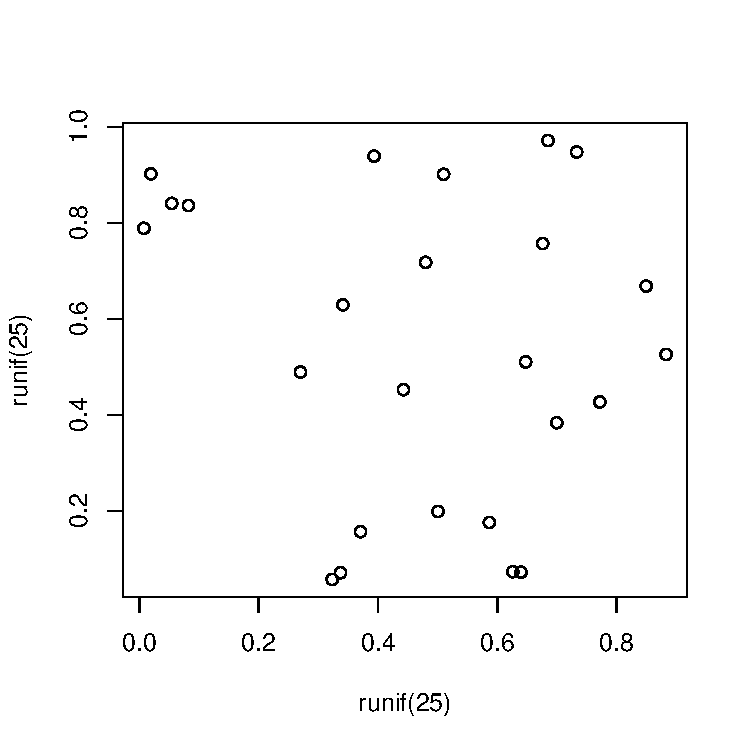
\includegraphics[width=0.5\linewidth]{CatchCompWaterCol_files/figure-latex/fig2-1} 

}

\caption{\label{fig2}A meaningless scatterplot.}\label{fig:fig2}
\end{figure}

\hypertarget{tables-coming-from-r}{%
\section{Tables coming from R}\label{tables-coming-from-r}}

Tables can also be generated using R chunks, as shown in Table
\ref{tab1} for example.

\begin{Shaded}
\begin{Highlighting}[]
\NormalTok{knitr}\SpecialCharTok{::}\FunctionTok{kable}\NormalTok{(}\FunctionTok{head}\NormalTok{(mtcars)[,}\DecValTok{1}\SpecialCharTok{:}\DecValTok{4}\NormalTok{], }
    \AttributeTok{caption =} \StringTok{"}\SpecialCharTok{\textbackslash{}\textbackslash{}}\StringTok{label\{tab1\}Caption centered above table"}
\NormalTok{)}
\end{Highlighting}
\end{Shaded}

\begin{longtable}[]{@{}lrrrr@{}}
\caption{\label{tab1}Caption centered above table}\tabularnewline
\toprule()
& mpg & cyl & disp & hp \\
\midrule()
\endfirsthead
\toprule()
& mpg & cyl & disp & hp \\
\midrule()
\endhead
Mazda RX4 & 21.0 & 6 & 160 & 110 \\
Mazda RX4 Wag & 21.0 & 6 & 160 & 110 \\
Datsun 710 & 22.8 & 4 & 108 & 93 \\
Hornet 4 Drive & 21.4 & 6 & 258 & 110 \\
Hornet Sportabout & 18.7 & 8 & 360 & 175 \\
Valiant & 18.1 & 6 & 225 & 105 \\
\bottomrule()
\end{longtable}

\hypertarget{references}{%
\section*{References}\label{references}}
\addcontentsline{toc}{section}{References}


\end{document}
